\begin{refsection}

\section{Thermal Conduction and Stress-Strain}
\label{sec:thermo_mech}

This section describes the core physics equations common to all FRED applications (FRED-ROD, FRED-OX, FRED-M-Na).  The equations are written first in differential (continuum) form and then in the finite-volume discretized form implemented in \texttt{HeatConduction.cpp} and \texttt{StressStrain.cpp}. It should be noted that the equations here present application agnostic equations, for example the correlation form of gap conductance, material property etc. are implemented in application specific code.

% =========================================================================
\subsection{Gap Pressure}
\label{sec:gap_pressure_rod}
% =========================================================================

The gap pressure $p_{gas}$ is a global algebraic variable common to all axial layers.  Two models are available, selected at the solver API level.

% -------------------------------------------------------------------------
\subsubsection{Prescribed Time-dependent Gap Pressure}
\label{sec:prescribed_pressure}
% -------------------------------------------------------------------------

The simplest model pins $p_{gas}$ to a user-supplied time series $p(t)$:
\begin{equation}
  p_{gas} = p(t).
  \label{eq:gpres_prescribed}
\end{equation}
The corresponding DAE residual is $r[0] = p_{gas} - p(t) = 0$.  A constant value is the most common case.

\paragraph{Typical use — liquid-bonded fuel.} In sodium-bonded metallic fuel (e.g.\ FRED-M-Na) the gap medium is liquid sodium.  Sodium is nearly incompressible, so the mechanical boundary condition at the cladding inner surface is set by the sodium \emph{system pressure}, not by a thermodynamic gas state.  The system pressure is approximately constant for a given operating condition and is prescribed directly via \texttt{set\_bond\_pressure(p\_MPa)}.

% -------------------------------------------------------------------------
\subsubsection{Gas Bond Pressure}
\label{sec:gas_bond_pressure}
% -------------------------------------------------------------------------

For gas-bonded fuel (e.g.\ He or Ar fill gas in FRED-ROD and FRED-OX) the pressure is determined by conservation of the molar fill-gas inventory $n$ under the ideal gas law:
\begin{equation}
  p_{gas} = \frac{n\,R}{v_T},
  \label{eq:gpres_ae}
\end{equation}
where $R = 8.314$~J/(mol\,K) is the universal gas constant.

\paragraph{Initial molar inventory.} The fill-gas moles are fixed from the as-fabricated conditions.  The user specifies the reference pressure $p_0$~[MPa] at room temperature $T_{ref} = 293.15$~K; together with the as-fabricated free volume $V_{free,0}$~[m$^3$] (gap annulus + central void + plenum),
\begin{equation}
  n = \frac{p_0 \times 10^6\; V_{free,0}}{R\,T_{ref}},
  \label{eq:mu0}
\end{equation}
and $n$ does not change during the simulation (no fission gas in FRED-ROD).

\paragraph{Temperature-weighted free volume.} The denominator $v_T$ is a temperature-weighted sum over all gas-filled regions:
\begin{multline}
  v_T = \frac{V_{pl}}{T_{pl}}
        + \sum_{j=0}^{n_z-1}
          \frac{\pi\,\Delta z_j\left(r_{ci,j}^2 - r_{fo,j}^2\right)}{T_{gap,j}} \\
        + \sum_{j=0}^{n_z-1}
          \frac{\pi\,\Delta z_j\,r_{fi,j}^2}{T_{ctr,j}}
  \label{eq:vT}
\end{multline}
where $V_{pl}$ is the plenum volume, $T_{pl}$ the plenum temperature, and $r_{fi,j}$, $r_{fo,j}$, $r_{ci,j}$ the deformed inner-fuel, outer-fuel, and inner-cladding radii of layer~$j$.  The central-void term vanishes for a solid pellet ($r_{fi,j} = 0$).

Two physical couplings follow directly from~\eqref{eq:gpres_ae}:
\begin{itemize}
\item \emph{Temperature rise} increases $v_T$ (larger $V/T$ terms) and therefore \emph{reduces} $p_{gas}$.
\item \emph{Gap closure} reduces the gap annulus volume, reducing $v_T$ and therefore \emph{increasing} $p_{gas}$ — which in turn raises the gas-pressure threshold that the contact pressure must exceed before the gap reopens.
\end{itemize}

\paragraph{FRED-OX.} In FRED-OX the molar inventory grows due to released fission gas: $n \to n + n_{fgr}(t)$, where $n_{fgr}$ is governed by its own ODE (Section~\ref{sec:fgr}).  Equation~\eqref{eq:gpres_ae} is otherwise identical; see Section~\ref{sec:gpres} for details.

% =========================================================================
\subsection{Thermal Conduction}
\label{sec:heat}
% =========================================================================

\subsubsection{Differential Form}

Assuming azimuthal symmetry, the transient heat conduction equation in cylindrical coordinates $(r,z)$ with volumetric heat generation $q'''$ is:

\begin{equation}
  \rho\, c_p \frac{\partial T}{\partial t}
  = \frac{1}{r}\frac{\partial}{\partial r}
    \!\left(r\,k\,\frac{\partial T}{\partial r}\right) + q'''
  \label{eq:heat_pde}
\end{equation}

where $\rho$ [kg/m$^3$] is the material density, $c_p$ [J/(kg\,K)] the isobaric heat capacity, $k$ [W/(m\,K)] the thermal conductivity, and $T$ [K] the temperature field.  Axial conduction is neglected in the current plane-strain implementation; each axial layer is solved independently.

\paragraph{Boundary conditions.}

\begin{itemize}
\item \emph{Symmetry at the fuel centre} (or inner hole gas pressure for annular pellets): $\partial T/\partial r = 0$ at $r = r_{fi}$ (solid pellet).
\item \emph{Fuel-cladding gap} at $r = r_{fo}$:
        \begin{equation}
          -k_f \frac{\partial T}{\partial r}\bigg|_{r_{fo}^-}
          = h_{gap}\,(T_f - T_c)
          \label{eq:gap_bc}
        \end{equation}
where $h_{gap}$ [W/(m$^2$\,K)] is the effective gap conductance (Section~\ref{sec:gap}) and $T_f, T_c$ are the fuel outer and cladding inner surface temperatures.
\item \emph{Coolant boundary} at $r = r_{co}$: two modes are available, reflecting the two principal use-cases for FRED.  In the first, FRED is coupled to an external sub-channel thermal-hydraulics (T-H) code that supplies the coolant temperature at all axial levels at all times; in the second, FRED uses in-built application sub-channel analysis and computes the coolant temperature internally.
        \begin{itemize}
\item \textbf{Dirichlet (prescribed temperature)} — FRED receives $T_{cool}(t)$ from the calling code or from a user-supplied time series and pins the outer cladding surface temperature directly:
                \begin{equation}
                  T\!\left(r_{co},t\right) = T_{cool}(t).
                  \label{eq:dirichlet_bc}
                \end{equation}
\item \textbf{Robin (convective HTC)} — a Newton's law of cooling condition is applied at the outer surface:
                \begin{equation}
                  -k_c\,\frac{\partial T}{\partial r}\bigg|_{r_{co}}
                  = h_{cool}(t)\,\bigl(T(r_{co},t) - T_{cool}(t)\bigr),
                  \label{eq:robin_bc}
                \end{equation}
where $h_{cool}$ [W/(m$^2$\,K)] is the cladding-to-coolant heat-transfer coefficient and $T_{cool}(t)$ is the \emph{local} bulk coolant temperature at the same axial position.  In the Robin mode both $h_{cool}$ and $T_{cool}$ are computed by an application-specific sub-channel model. Sub-channel variables (coolant properties, channel geometry, HTC correlation) are platform-specific; the FRED-M-Na sodium sub-channel implementation is described in Section~\ref{sec:subchannel_mna}.
        \end{itemize}
\end{itemize}

\subsubsection{Gap Conductance Model}
\label{sec:gap}

The thermal boundary condition at the fuel--cladding interface, Eq.~\eqref{eq:gap_bc}, requires an effective interfacial conductance $h_{gap}$. The physical form depends on whether the gap medium is a gas (free surface) or a liquid bond.

% ---- gas-filled gap ----
\paragraph{Gas-filled gap (free surface).} When the gap contains a cover gas (He, Ar, or a fission-gas/cover-gas mixture), the fuel outer surface is a \emph{free surface}: it carries only the normal gas pressure $p_{gas}$ and no tangential traction.  Heat transfer across the gas layer is limited by the low gas thermal conductivity and by a temperature discontinuity at each solid surface (temperature-jump effect).  The general form of the gas-gap conductance is:
\begin{equation}
  h_{gap}^{\mathrm{gas}} = \frac{k_{gas}(\bar{T})}{\delta + g_f + g_c} + h_{rad}
  \label{eq:hgap_gas}
\end{equation}
where
\begin{itemize}
\item $k_{gas}(\bar{T})$ is the gas thermal conductivity at mean gap temperature $\bar{T} = \tfrac{1}{2}(T_f + T_c)$,
\item $\delta = r_{ci} - r_{fo}$ is the physical gap width (Eq.~\eqref{eq:gap_ae}),
\item $g_f$ and $g_c$ are the temperature-jump distances at the fuel and cladding surfaces, accounting for partial accommodation of gas molecules at each wall, and
\item $h_{rad} = \sigma_{SB}\,\varepsilon_{\mathrm{eff}}\, (T_f^2 + T_c^2)(T_f + T_c)$ is the radiative contribution across the cavity, with $\sigma_{SB}$ the Stefan--Boltzmann constant and $\varepsilon_{\mathrm{eff}}$ the effective emissivity.
\end{itemize}
The gap pressure $p_{gas}$ is governed by the ideal-gas model (Section~\ref{sec:gas_bond_pressure}).  The variables $k_{gas}$, $g_f$, $g_c$, and $\varepsilon_{\mathrm{eff}}$ are application-specific correlations for example Section~\ref{sec:gap_ox} (FRED-OX).

% ---- liquid-filled gap ----
\paragraph{Liquid-filled gap.} When the gap is filled with a liquid bond (e.g.\ liquid sodium in FRED-M-Na), no temperature-jump effect because the liquid maintains continuous thermal contact with both solid surfaces.  The conductance reduces to:
\begin{equation}
  h_{gap}^{\mathrm{liq}} = \frac{k_{liq}(\bar{T})}{\delta}
  \label{eq:hgap_liq}
\end{equation}
where $k_{liq}(\bar{T})$ is the thermal conductivity of the liquid bond. Because $k_{\mathrm{Na}} \approx 60$--$80$\,W/(m\,K) at typical fast-reactor temperatures compared with $k_{\mathrm{He}} \approx 0.15$--$0.35$\,W/(m\,K) for helium, the liquid-bonded gap conductance is one to two orders of magnitude higher than a gas-bonded gap of equal width.

The mechanical boundary condition at a liquid-filled gap retains the same \emph{free-surface pressure} form as the gas case (open-gap conditions in Section~\ref{sec:stress_strain}).  Application-specific closures for $k_{liq}(\bar{T})$ are described in Section~\ref{sec:gap_mna} (FRED-M-Na).

\subsubsection{Finite-Volume Discretization}

The pellet cross-section is divided into $n_f$ concentric rings of uniform radial width $\Delta r_f = (r_{fo} - r_{fi})/(n_f - 1)$, and the cladding into $n_c$ rings of width $\Delta r_c = (r_{co} - r_{ci})/(n_c - 1)$.  Nodes are placed at ring centroids (vertex-centred scheme).

An energy balance over ring $i$ (cross-sectional area $A_i$ [m$^2$]) gives the ODE for fuel ring temperatures ($i = 0,\ldots,n_f - 1$):

\begin{equation}
  \rho_f c_{p,f}(T_i)\,A_i\,\frac{dT_i}{dt}
  = q'''\,A_i + Q_{i-1 \to i} - Q_{i \to i+1}
  \label{eq:heat_ode_fuel}
\end{equation}

and for inner cladding rings ($i = n_f,\ldots,n_f + n_c - 2$, no volumetric generation):

\begin{equation}
  \rho_c c_{p,c}(T_i)\,A_i\,\frac{dT_i}{dt}
  = Q_{i-1 \to i} - Q_{i \to i+1}
  \label{eq:heat_ode_clad}
\end{equation}

The inter-ring heat flow per unit axial length [W/m] between nodes $i$ and $i+1$ is evaluated using the interface-averaged conductivity at half-node radius $\bar{r}_i$:

\begin{equation}
  Q_{i \to i+1} = k\!\left(\tfrac{T_i + T_{i+1}}{2}\right)
                  \frac{T_i - T_{i+1}}{\Delta r} \cdot 2\pi\bar{r}_i
  \label{eq:Qflux}
\end{equation}

The outer cladding node carries an algebraic equation (AE) whose form depends on the active BC mode:

\begin{equation}
  \text{Dirichlet:}\quad T_{n_f+n_c-1} = T_{cool}(t)
  \label{eq:outerBC_dirichlet}
\end{equation}
\begin{equation}
  \text{Robin:}\quad Q_{n_f+n_c-2 \to n_f+n_c-1}
    = h_{cool}\cdot 2\pi r_{co}\cdot\bigl(T_{n_f+n_c-1} - T_{cool}(t)\bigr)
  \label{eq:outerBC_robin}
\end{equation}

In both cases the outer node equation is algebraic, so the equation count is unchanged.  The Robin form sets the conductive flux arriving at the outer ring equal to the convective flux leaving to the coolant; $h_{cool}$ and $T_{cool}$ are supplied by the application-specific sub-channel model.

The fuel-clad gap heat flow (index $i = n_f - 1$) is:
\begin{equation}
  Q_{gap} = h_{gap}\,(T_{n_f-1} - T_{n_f}) \cdot 2\pi r_{fo}
  \label{eq:Qgap}
\end{equation}

\paragraph{Auxiliary algebraic equations.} The DAE system carries four auxiliary scalar variables — volumetric power $q'''$, gap width $\delta$, contact pressure $p_{fc}$, and gap conductance $h_{gap}$ — each pinned by its own algebraic equation:
\begin{align}
  q'''    &= q'''(t)
            \label{eq:qqv_ae}\\
  \delta  &= r_{ci} - r_{fo}
            \label{eq:gap_ae}\\
  p_{fc}  &= \begin{cases}
               0                  & \text{(open gap)}   \\
               |\sigma_r^{(0)}|   & \text{(closed gap)}
             \end{cases}
            \label{eq:pfc_ae}\\
  h_{gap} &= h_{gap}(\,\cdot\,)
            \label{eq:hgap_ae}
\end{align}
where $r_{ci}$ and $r_{fo}$ are the deformed cladding inner and fuel outer radii, and $\sigma_r^{(0)}$ is the cladding inner surface radial stress. The gap conductance closure~\eqref{eq:hgap_ae} is application-specific (Section~\ref{sec:gap}).

\paragraph{Equation count.} The thermal block contributes $4 + n_f + n_c$ equations per axial layer:
\begin{itemize}
\item 4 auxiliary AEs: power density~\eqref{eq:qqv_ae}, gap width~\eqref{eq:gap_ae}, contact pressure~\eqref{eq:pfc_ae}, and gap conductance~\eqref{eq:hgap_ae}.
\item $n_f$ fuel temperature ODEs~\eqref{eq:heat_ode_fuel}.
\item $(n_c - 1)$ inner cladding temperature ODEs~\eqref{eq:heat_ode_clad}.
\item 1 outer cladding AE — either the Dirichlet form~\eqref{eq:outerBC_dirichlet} or the Robin form~\eqref{eq:outerBC_robin}; the equation count is the same for both modes.
\end{itemize}
The last two groups together give $n_c$ cladding equations, so the total is $4 + n_f + n_c$, regardless of which coolant BC is active.

The material thermal conductivity $k(T)$, heat capacity $c_p(T)$, and density $\rho$ formulations are application specific e.g. in FUEL-ROD, users can specify arbitrary correlations while in FRED-OX, correlations specific to MOX are used (~Section:\ref{sec:mox_correlations}).

% =========================================================================
\subsection{Stress-Strain}
\label{sec:stress_strain}
% =========================================================================

\subsubsection{Differential Form}

FRED applies the plane-strain / plane-stress assumption (all axial layers deform independently with a uniform axial strain $\varepsilon_z$), the governing equations for a cylindrical body in cylindrical coordinates $(r,\theta,z)$ are as follows:

\paragraph{Strain-displacement relations.}

In a thin circular ring of radius $r$ with radial displacement $u$. The radial strain a.k.a. the stretching of the ring in the radial direction is
\begin{equation}
  \varepsilon_r = \frac{du}{dr}.
\end{equation}

Taking a small arc length subtending an angle $d \theta$ of original length $ds = r d\theta$ and final lenght $ds' = (r + u) d \theta$, the strain of that arc is
\begin{equation}
  \varepsilon_\theta = \frac{ds' - ds}{ds} = \frac{(r + u)d \theta - r d\theta}{r d \theta} = \frac{u}{r}. 
\end{equation}

\begin{align}
  \varepsilon_\theta &= \frac{u}{r}, \quad
  \varepsilon_r = \frac{du}{dr}, \quad
  \varepsilon_z = \text{const (per layer)}
  \label{eq:strain_disp}
\end{align}

\paragraph{Radial compatibility.}
\begin{equation}
  \frac{d(r\,\varepsilon_\theta)}{dr} = \varepsilon_r
  \label{eq:compat_cont}
\end{equation}

\paragraph{Radial equilibrium.}
\begin{equation}
  \frac{d(r\,\sigma_r)}{dr} = \sigma_\theta
  \label{eq:equil_cont}
\end{equation}

\paragraph{Thermal strain.} The total strain is decomposed into elastic and thermal parts, $\varepsilon = \varepsilon^{el} + \varepsilon^{th}$, where the isotropic thermal expansion strain is
\begin{equation}
  \varepsilon^{th}(T) = \alpha_{\mathrm{CTE}}\,(T - T_{\mathrm{ref}})
  \label{eq:thermal_strain}
\end{equation}
with $\alpha_{\mathrm{CTE}}$ [1/K] the linear coefficient of thermal expansion and $T_{\mathrm{ref}}$ the stress-free reference temperature.

% Figure~\ref{fig:ring_compat_equil} gives an intuitive differential-ring view
% of these two constraints: non-uniform radial displacement across the ring
% enforces strain compatibility, while radial traction variation across the same
% ring enforces radial stress equilibrium.

% \begin{figure}[htbp]
%   \centering
%   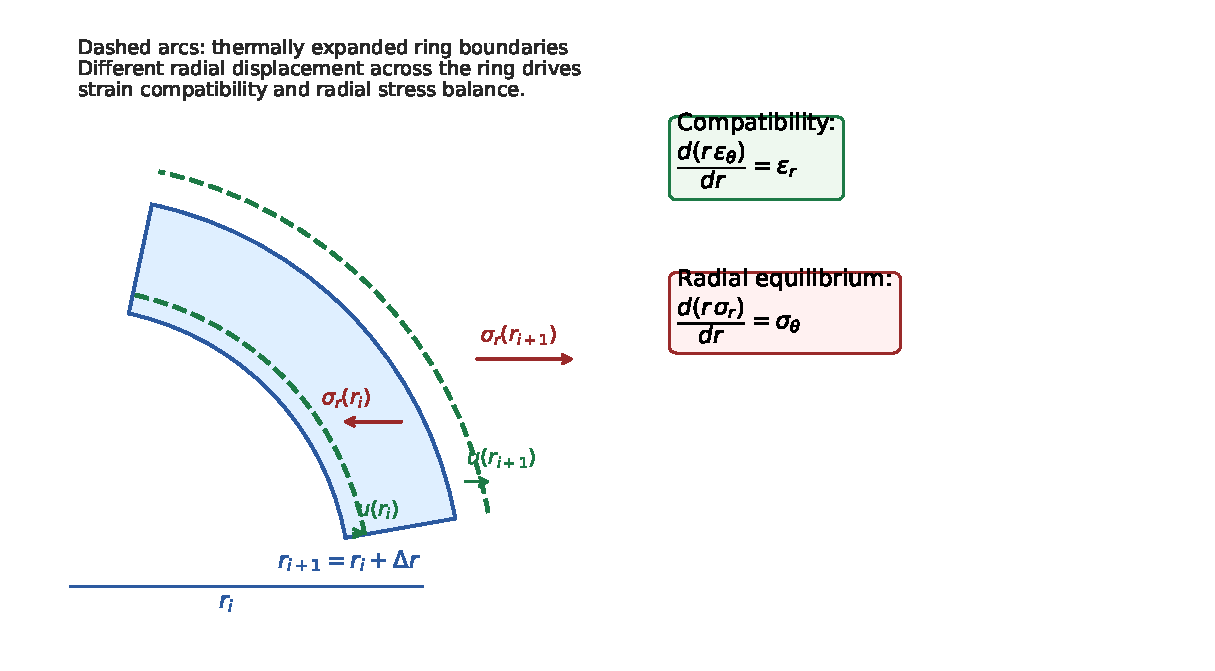
\includegraphics[width=0.90\textwidth]{images/mech_ring_compatibility.pdf}
%   \caption{Differential ring interpretation of radial strain compatibility and
%            radial stress equilibrium. Dashed arcs indicate differential thermal
%            expansion of inner/outer ring boundaries; radial traction arrows
%            indicate the balance represented by
%            $\frac{d(r\,\sigma_r)}{dr}=\sigma_\theta$.}
%   \label{fig:ring_compat_equil}
% \end{figure}

\paragraph{Thermo-elastic constitutive law (Hooke's law with thermal expansion).} Using the thermal strain~\eqref{eq:thermal_strain}, the elastic strains relate to stresses via:

\begin{align}
  E\,(\varepsilon_\theta - \varepsilon^{th}) &= \sigma_\theta - \nu(\sigma_r + \sigma_z)
  \label{eq:hooke_h}\\
  E\,(\varepsilon_r     - \varepsilon^{th}) &= \sigma_r     - \nu(\sigma_\theta + \sigma_z)
  \label{eq:hooke_r}\\
  E\,(\varepsilon_z     - \varepsilon^{th}) &= \sigma_z     - \nu(\sigma_\theta + \sigma_r)
  \label{eq:hooke_z}
\end{align}

where $E$ [MPa] is Young's modulus and $\nu$ Poisson's ratio.


\paragraph{Boundary conditions.}

Fuel (3 conditions) and cladding (3 conditions) each carry three boundary equations, giving six in total.

\emph{Fuel (BC-1, BC-2, BC-3):}
\begin{itemize}
\item \emph{BC-1 — Axial force balance}:
        \begin{itemize}
\item Open gap: $\displaystyle\sum_{i=0}^{n_f-1} A_{f,i}\,\sigma_{z,f}^{(i)} + A_{z,f}\,p_{gas} = 0$.
\item Closed gap (combined fuel+clad): $\displaystyle\sum_{i=0}^{n_f-1} A_{f,i}\,\sigma_{z,f}^{(i)} + \sum_{i=0}^{n_c-1} A_{c,i}\,\sigma_{z,c}^{(i)} + \pi r_{co}^2\,p_{cool} = 0$.
        \end{itemize}
\item \emph{BC-2 — Inner radial surface} (solid pellet): symmetry $\sigma_r^{(0)} = \sigma_\theta^{(0)}$.  For an annular pellet: $\sigma_r^{(0)} = -p_{gas}$.
\item \emph{BC-3 — Outer radial surface / gap interface}:
        \begin{itemize}
\item Open gap: $\sigma_r^{(n_f-1)} = -p_{gas}$.
\item Closed gap: axial strain compatibility $\varepsilon_z^{f} = \varepsilon_z^{c}$.
        \end{itemize}
\end{itemize}

\emph{Cladding (BC-1, BC-2, BC-3):}
\begin{itemize}
\item \emph{BC-1 — Axial / interface condition}:
        \begin{itemize}
\item Open gap (cladding axial force balance): $\displaystyle\sum_{i=0}^{n_c-1} A_{c,i}\,\sigma_{z,c}^{(i)} + \pi r_{co}^2\,p_{cool} - \pi r_{ci}^2\,p_{gas} = 0$.
\item Closed gap (radial traction continuity at fuel–clad interface): $\sigma_{r,f}^{(n_f-1)} = \sigma_{r,c}^{(0)}$.
        \end{itemize}
\item \emph{BC-2 — Inner radial surface}:
        \begin{itemize}
\item Open gap: $\sigma_r^{(0)} = -p_{gas}$.
\item Closed gap: gap width locked at surface roughness $\delta = \delta_{rough}$.
        \end{itemize}
\item \emph{BC-3 — Outer radial surface}: $\sigma_r^{(n_c-1)} = -p_{cool}$.
\end{itemize}

Here $A_{z,f} = \pi r_{fi}^2$ for annular fuel (zero for a solid pellet), so gas loading on the fuel end appears only when a central hole is present.
\label{eq:axial_balance}

\subsubsection{Finite-Volume Discretization}

Each ring~$i$ is treated as a finite-volume cell with area $A_i = \pi(r_{i+1}^2 - r_i^2)$.  The unknown strains and stresses are defined at the node location $r_i$.  The compatibility equation~\eqref{eq:compat_cont} integrated over a ring of width $\Delta r$ between nodes $i$ and $i+1$ gives:

\begin{equation}
  \Delta r\;\bar{\varepsilon}_r + r_i\,\varepsilon_\theta^{(i)}
  - r_{i+1}\,\varepsilon_\theta^{(i+1)} = 0
  \label{eq:compat_disc}
\end{equation}

where $\bar{\varepsilon}_r = \tfrac{1}{2}(\varepsilon_r^{(i)} + \varepsilon_r^{(i+1)})$.  The stress equilibrium equation \eqref{eq:equil_cont} over the same ring is:

\begin{equation}
  \Delta r\;\bar{\sigma}_\theta + r_i\,\sigma_r^{(i)}
  - r_{i+1}\,\sigma_r^{(i+1)} = 0
  \label{eq:equil_disc}
\end{equation}

with $\bar{\sigma}_\theta = \tfrac{1}{2}(\sigma_\theta^{(i)} + \sigma_\theta^{(i+1)})$.  At each node, the thermal expansion strain is also pinned to the local temperature by an algebraic equation,
\begin{equation}
  \varepsilon^{th}_i = \varepsilon^{th}(T_i),
  \label{eq:thexp_disc}
\end{equation}
where $\varepsilon^{th}(T)$ is defined in~\eqref{eq:thermal_strain}.  Together with the three Hooke's law equations~\eqref{eq:hooke_h}--\eqref{eq:hooke_z} and the boundary conditions listed above, each body with $n$ nodes contributes equations in three groups:
\begin{itemize}
\item $4n$ at-node equations: thermal expansion AE~\eqref{eq:thexp_disc} plus Hooke's law~\eqref{eq:hooke_h}--\eqref{eq:hooke_z} in $\theta$, $r$, $z$.
\item $2(n-1)$ inter-node equations: one compatibility~\eqref{eq:compat_disc} and one equilibrium~\eqref{eq:equil_disc} per adjacent node pair ($n-1$ pairs for $n$ nodes).
\item 3 boundary condition equations: inner radial surface, outer radial surface / gap interface, and axial force balance.
\end{itemize}
Each body therefore contributes $4n + 2(n-1) + 3 = 6n + 1$ equations. Summing fuel ($n = n_f$) and cladding ($n = n_c$):
\begin{equation}
  (6\,n_f + 1) + (6\,n_c + 1) = 6(n_f + n_c) + 2.
  \label{eq:mech_neq}
\end{equation}

\paragraph{Gap state machine.} The gap opens and closes as the fuel expands radially.  The event is detected by SUNDIALS IDA root-finding:

\begin{itemize}
\item \emph{Closure root}: $g_1 = \delta - \delta_{thresh} = 0$, $\delta_{thresh} = \rho_f + \rho_c$.
\item \emph{Reopening root}: $g_2 = p_{fc} - p_{gas} = 0$.
\end{itemize}

The closure root tracks the mechanical closure between the fuel pellet and the cladding, while the re-opening root tracks when the pressure in the gap exceeds the contact pressure, causing re-opening. Upon gap closure, the boundary-condition set switches as follows:

\begin{align}
  \text{Fuel outer BC (open)}\quad &\sigma_{r,f}^{(n_f-1)} = -p_{gas}
  \quad\Longrightarrow\quad
  \text{(closed)}\; \varepsilon_{z,f} - \varepsilon_{z,c} = 0 \\
  \text{Clad inner BC (open)}\quad &\sigma_{r,c}^{(0)} = -p_{gas}
  \quad\Longrightarrow\quad
  \text{(closed)}\; \delta - \delta_{rough} = 0
\end{align}

and the closed-gap contact interface additionally enforces radial traction continuity,
\begin{equation}
  \sigma_{r,f}^{(n_f-1)} - \sigma_{r,c}^{(0)} = 0.
\end{equation}

In the axial force balance, the branch switch is explicit:
\begin{itemize}
\item \emph{Open gap} (separate fuel and clad axial equilibrium):
        \begin{align}
          \sum_{i=0}^{n_f-1} A_{f,i}\,\sigma_{z,f}^{(i)} + A_{z,f}\,p_{gas} &= 0, \\
          \sum_{i=0}^{n_c-1} A_{c,i}\,\sigma_{z,c}^{(i)}
          + \pi r_{co}^2\,p_{cool} - \pi r_{ci}^2\,p_{gas} &= 0.
        \end{align}
\item \emph{Closed gap} (shared fuel+clad axial equilibrium):
        \begin{equation}
          \sum_{i=0}^{n_f-1} A_{f,i}\,\sigma_{z,f}^{(i)}
          + \sum_{i=0}^{n_c-1} A_{c,i}\,\sigma_{z,c}^{(i)}
          + \pi r_{co}^2\,p_{cool} = 0.
        \end{equation}
\end{itemize}
Here $A_{z,f}=\pi r_{fi}^2$ for annular fuel (and $A_{z,f}=0$ for a solid pellet), so gas loading on the fuel axial end appears only when a central hole exists.

\paragraph{Equation-of-state summary.} Including the one global gas-pressure AE~\eqref{eq:gpres_ae} and the per-layer thermal and mechanical blocks, the total equation count is
\begin{multline}
  \underbrace{1}_{\text{global }p_{gas}}
  \;+\;
  n_z\!\left[
    \underbrace{(4 + n_f + n_c)}_{\text{thermal}}
    +\;
    \underbrace{6(n_f + n_c) + 2}_{\text{mechanical}}
  \right] \\
  =\; 1 + n_z\bigl[7(n_f + n_c) + 6\bigr]
  \;\equiv\; 7(n_f + n_c) + 7 \;\text{(per layer + global).}
  \label{eq:neq_total}
\end{multline}

The state vector is ordered as follows:
\begin{equation}
  \mathbf{y} =
  \left[
  \begin{array}{cl}
    p_{gas}
      & \text{1 global AE~\eqref{eq:gpres_ae}} \\[4pt]
    \hline \\[-7pt]
    q'''_0,\;\delta_0,\;p_{fc,0},\;h_{gap,0}
      & \text{layer 0: 4 thermal AEs~\eqref{eq:qqv_ae}--\eqref{eq:hgap_ae}} \\
    T^{(0)}_0,\;\ldots,\;T^{(0)}_{n_f+n_c-1}
      & \text{layer 0: $n_f+n_c$ temperatures~\eqref{eq:heat_ode_fuel}--\eqref{eq:outerBC_dirichlet}} \\
    \varepsilon^{th}_{f,0},\ldots,\varepsilon^{h}_{f,0},\ldots,\varepsilon_{fz},\,
    \sigma^{h}_{f,0},\ldots
      & \text{layer 0: fuel mechanics ($6n_f+1$)} \\
    \varepsilon^{th}_{c,0},\ldots,\varepsilon^{h}_{c,0},\ldots,\varepsilon_{cz},\,
    \sigma^{h}_{c,0},\ldots
      & \text{layer 0: clad mechanics ($6n_c+1$)} \\[4pt]
    \hline \\[-7pt]
    \multicolumn{2}{c}{\vdots} \\[4pt]
    \hline \\[-7pt]
    q'''_{n_z-1},\;\delta_{n_z-1},\;\ldots
      & \text{layer $n_z-1$: (same structure)}
  \end{array}
  \right]
  \label{eq:state_vec}
\end{equation}

\printbibliography[heading=subbibliography,title={References}]
\end{refsection}
